\documentclass[paper=letter, fontsize=11pt]{scrartcl} % A4 paper and 11pt font size
\newcommand{\horrule}[1]{\rule{\linewidth}{#1}} % Create horizontal rule command with 1 argument of height
\setlength{\parskip}{1em}
\setlength{\parindent}{3em}

\usepackage{amsmath}
\usepackage{geometry}
 \geometry{
 bottom=1in,
 right=1in,
 left=1in,
 top=1in,
 }
 
 \usepackage[flushleft]{threeparttable}
\usepackage[capposition=top]{floatrow}

\usepackage{graphicx}

\title{	
\normalfont \normalsize 
\horrule{0.5pt} \\[0.4cm] % Thin top horizontal rule
 \large{{\textbf{ECON 293 Homework 1: Commentary}}} \\ % The assignment title
\horrule{2pt} \\[0.5cm] % Thick bottom horizontal rule
}

\author{\small{Jack Blundell, Spring 2017}} % Your name

\date{} % Today's date or a custom date

\begin{document}

\maketitle % Print the title

In this writeup I discuss results and include some key figures. Many further figures and all code are provided in the attached .html file. I worked with Luis Armona on the code and this commentary is written individually.

\section{}

We chose to use data from ``Does Price Matter in Charitable Giving?
Evidence from a Large-Scale Natural Field Experiment", by Dean Karlan and John List (AER 2007). First we estimate the average treatment effect, pooling all treatments, on outcome variable total donation given via regression. We find a treatment effect of $0.1536$, with a 95\% confidence interval of $-0.0082, 0.3154 $, consistent with the results in the paper.

\section{}

Our selection rule uses the fact that in the paper, it is demonstrated that treatment effects are highest among states which voted for Bush in the most recent election, and that this effect is biggest for the most marginal states. The probability of selection is chosen to be:
\begin{align*}
  \psi &= log(X_3 + sqrt(X_3 ^ 2 + 1)) \\
Pr(S|W,X) &= (1-W)*(X_2+1)*(acos(X_1)*atan(X_1) )/3 + 
      W*(.01+(-.01*\psi^5 + \psi^3)/300)
\end{align*}
Here, $W$ is treatment, $X_1$ is the percentage who voted for Bush in the previous election, and $X_1,X_2$ are other covariates found to be correlated with treatment effects. This is a highly non-linear function involving several variables and hence unlikely to be recoverable by standard propensity score methods. \ref{select} shows the shape of this function across proportion of Bush voters for a number of other covariate values.

\begin{figure}[!ht]
\center
\caption{Selection rule  \label{select}}
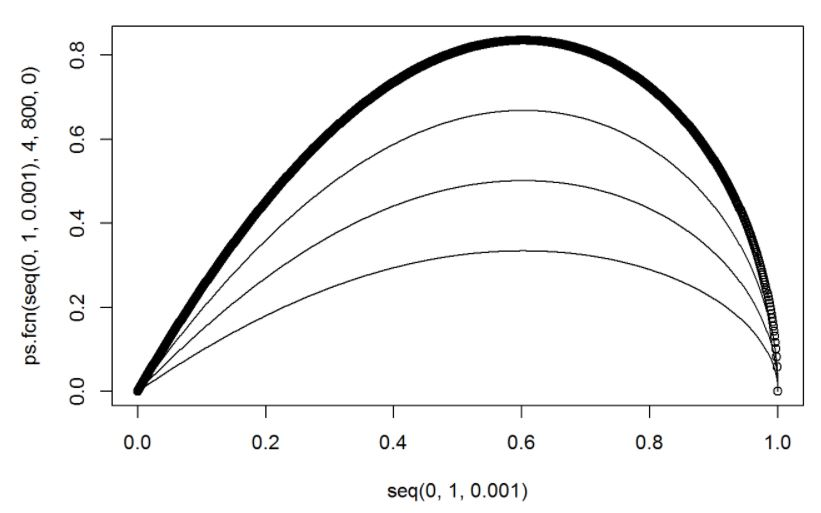
\includegraphics[scale=0.8]{figs/select_shape.jpg}
\floatfoot{Notes: x-axis is number of votes won by Bush in previous election. This graph shows the shape of our selection rule for a number of different covariate values.}
\end{figure}

We calculate $Pr(S|W,X)$ for each observation, and use a uniform random number generator to drop observations based on this. This selection means that we no-longer have a randomized experiment. Table \ref{treat} shows the full set of treatment effects estimated in this homework. The first row shows the simple OLS on the full sample\footnote{note that this does not coincide with the previously-given estimate since we have restricted the sample to eliminate observations with missing covariates}. This could be considered the `true' treatment effect, i.e. the treatment effect without selection. The estimate below of $0.3627$ shows that when we restrict the sample according to our selection rule, the estimated treatment effect increases.

\begin{table}[htbp]  \small
 \centering
  \begin{threeparttable}  
\caption{Estimated treatment effects \label{treat}}\begin{tabular}{l*{1}{c}}
\hline
Estimator           &     Estimated treatment effect     
\rule{0pt}{4ex}  \\
\hline\hline
Full sample simple OLS &  0.1661 \\
\hline
Restricted sample simple OLS &  0.3627 \\
PS Weighting          &            0.1665 \\
OLS w/ Controls       &            0.1225 \\ \hline
Traditional DR OLS w/ IPS Weights & 0.0884 \\
Regularized PS Weighted &             0.1792 \\
Classic Double Robust w/ Regularized PS & 0.1574 \\
Direct Lasso on Outcome &   0.1138 \\ \hline
Double Selection       &    0.1018 \\
Lasso Residual-on-Residual & 0.1123 \\
Residual balancing & \\
\end{tabular}
\begin{tablenotes}
\item Notes: This table shows the various treatment effects estimated throughout this homework
    \end{tablenotes}
  \end{threeparttable}
\end{table}

Overlap is demonstrated in Figure \ref{overlap}, which shows the true propensity scores for the treatment and control groups in the restricted sample. 


\begin{figure}[!ht]
\center
\caption{Overlap  \label{overlap}}
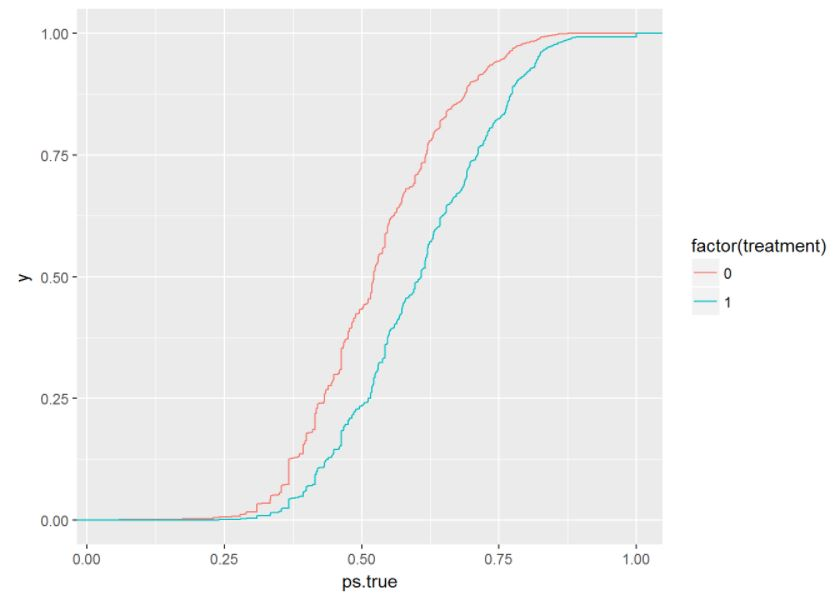
\includegraphics[scale=0.8]{figs/overlap.jpg}
\floatfoot{Notes: This graph shows the true propensity scores among treatment and control groups.}
\end{figure}

These true propensity scores are calculated by Bayes theorem, combining our selection rule with the (unconditional) probability of treatment in the original sample.

Figure \ref{bias} is the histogram of the bias function as given in Athey, Imbens, Pham and Wager (2017). The expected bias is $0.061$. As expected, since we have disproportionately included the treated with high treatment effects, the bias is generally positive. If we were to treat this as a random experiment, our treatment effect estimate would be biased upwards. This is consistent with what we see in Table \ref{treat}.

\begin{figure}[!ht]
\center
\caption{Bias Function  \label{bias}}
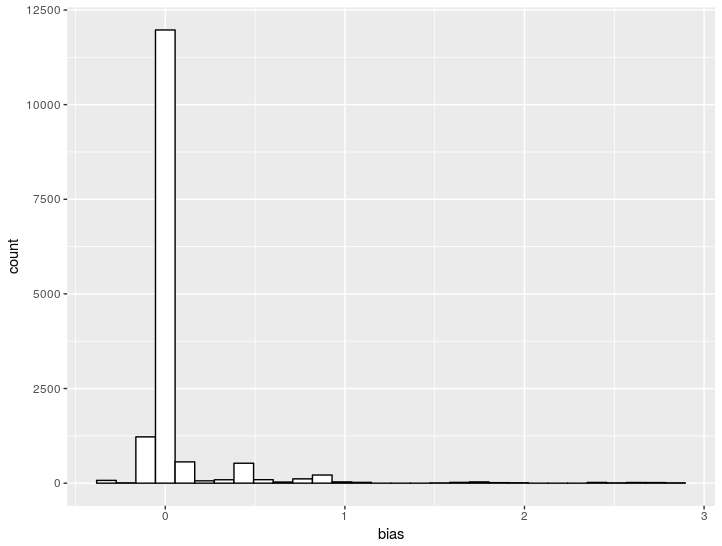
\includegraphics[scale=0.8]{figs/bias.jpg}
\floatfoot{Notes: This graph shows the distribution of the bias, as given in Athey, Imbens, Pham and Wager (2017).}
\end{figure}

\section{}

\section{}


\end{document}
